Let $X_i$ denote the random variable function for the $i$th coin $i\in\{1,2,3,4\}$.\\
$X_i\in(0,1)$ where 0 represents head and 1 represents tail $i\in\{1,2,3,4\}$.
\\[5pt]
\begin{tabular}{|c|c|c|}
\hline
     &Head&Tail  \\
     \hline
     $X_i=k$&0&1\\
     \hline
\end{tabular}
\begin{equation}\label{ec29-1:coin}
\Pr(X_i=k)=\dfrac{1}{2} 
\end{equation}
$k\in\{0,1\}$ and $i\in\{1,2,3,4\}$.
\\
Let $Y$ denote the random variable function for the dice.\\
$Y\in(1,2,3,4,5,6)$ where 1 represents dice showing 1 and so on.
\\[5pt]
\begin{tabular}{|c|c|c|c|c|c|c|}
\hline
     Dice number&1&2&3&4&5&6  \\
     \hline
     $Y=k$&1&2&3&4&5&6\\
     \hline
\end{tabular}
\\
\begin{equation}\label{ec29-1:dice}
\Pr(Y=k)=\dfrac{1}{6} 
\end{equation}
$k\in\{1,2,3,4,5,6\}$.
\\[20pt]
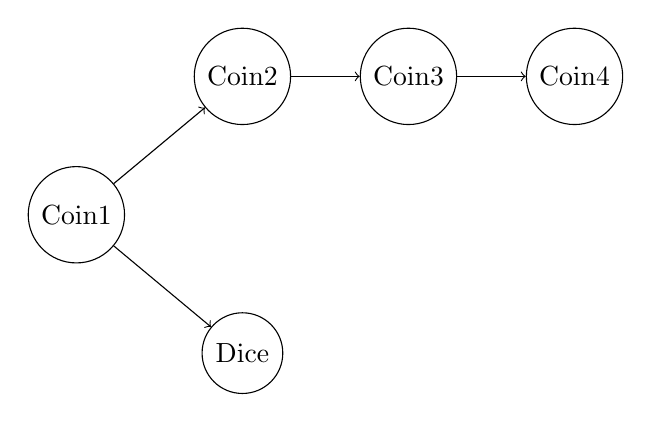
\begin{tikzpicture}
      [sibling distance=10em,level distance=6em, grow=right,
      every node/.style={shape=circle,draw,align=center},->]
      \node{Coin1}
   child
   {
    node{Dice}
   }
   child
   {
    node{Coin2}
      child
      {
        node{Coin3}
        child
      {
        node{Coin4}
      }
      }
    };
\end{tikzpicture}
Let B denote the event that out of last three coins, only one shows tail. \\
By Binomial Distribution,
\begin{align}
\Pr(B)&=\comb{3}{1}\brak{{\dfrac{1}{2}}}^3
\\[\parskip]
&=\dfrac{3}{8}
\end{align}
%
Since tossing a coin and rolling a dice are independent events,
\begin{equation}\label{ec29-1:independent theorem}
\Pr( (X_i=k),(Y=l) )= \Pr(X_i=k)\cdot \Pr(Y=l)
\end{equation}
$k\in\{0,1\}$ and $l\in\{1,2,3,4,5,6\}$.

Let A denote the event that the score is 2.

Clearly,
\begin{align}
\Pr(A)\nonumber&=\Pr(Y=2|X_1=0)\cdot \Pr(X_1=0) \\
    &+ \Pr(B|X_1=1)\cdot \Pr(X_1=1) 
\\[\parskip]
&=\Pr( (X_1=0),(Y=2) ) + \Pr( (X_1=1), B)
\\[\parskip]
&=\Pr(X_1=0)\cdot \Pr(Y=2)+ \Pr(X_1=1) \cdot \Pr(B)
\\[\parskip]
&=\dfrac{13}{48}
\end{align}
We have to find $\Pr(X_1=0|A)$
\begin{align}
\Pr(X_1=0|A)&=\dfrac{\Pr(A,(X_1=0) )}{\Pr(A)}
\\[\parskip]
&=\dfrac{\Pr(X_1=0)\cdot \Pr(Y=2)}{\Pr(A)}
\\[\parskip]
&=0.31
\end{align}

\textbf{Therefore, required probability = 0.31}

